\documentclass[tikz,margin=2mm]{standalone}
\usepackage{tikz}
\tikzset{
  hole/.style = {fill = #1, circle, minimum width = 2.5mm, inner sep = 0mm},
  wire/.style = {draw = #1, line width = .5mm},
  label/.style = {rotate = #1, black!50!white, anchor = center},
}
\begin{document}
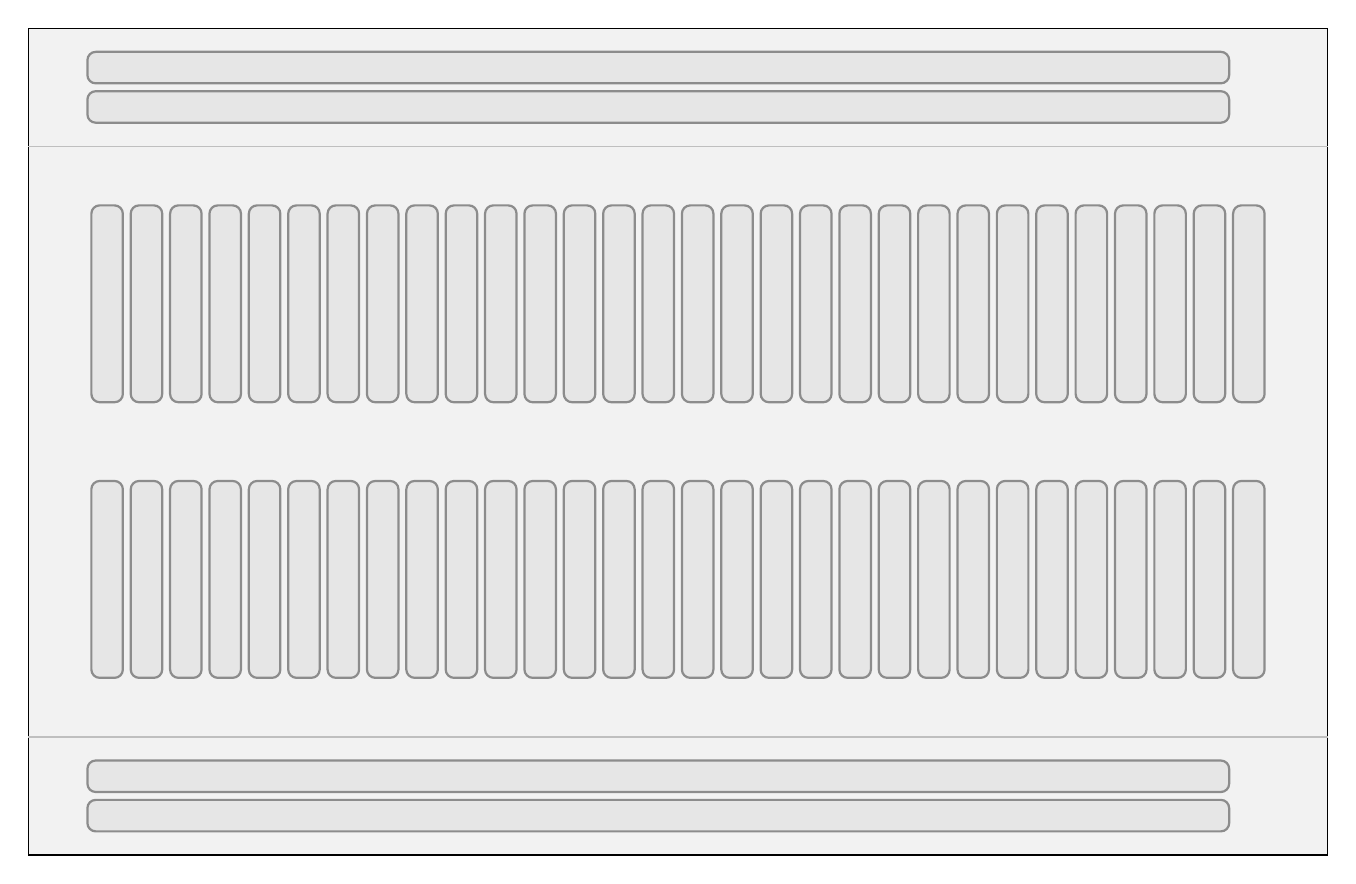
\begin{tikzpicture}[x=5mm,y=5mm]
  \draw[fill=black!05!white] (-1,-4) rectangle (32,17);
  \draw[wire=gray!50, line width = 0.5] (-1,14) -- (32,14);
  \draw[wire=gray!50, line width = 0.5] (-1,-1) -- (32,-1);
  
  \foreach \xi in {0,...,29}{
    \draw[rounded corners=3pt, thick, draw=gray!90, fill=gray, fill opacity=0.1] (\xi+0.6,7.5) rectangle (\xi+1.4,12.5);
    \draw[rounded corners=3pt, thick, draw=gray!90, fill=gray, fill opacity=0.1] (\xi+0.6,0.5) rectangle (\xi+1.4,5.5);
  }
  
  \draw[rounded corners=3pt, thick, draw=gray!90, fill=gray, fill opacity=0.1] (0.5,15.6) rectangle (29.5,16.4);
  \draw[rounded corners=3pt, thick, draw=gray!90, fill=gray, fill opacity=0.1] (0.5,14.6) rectangle (29.5,15.4);
  
  \draw[rounded corners=3pt, thick, draw=gray!90, fill=gray, fill opacity=0.1] (0.5,-3.4) rectangle (29.5,-2.6);
  \draw[rounded corners=3pt, thick, draw=gray!90, fill=gray, fill opacity=0.1] (0.5,-2.4) rectangle (29.5,-1.6);
\end{tikzpicture}
\end{document}